\section{Design}

In order to achieve deterministic latencies, we need to ensure both hardware and software usage is deterministic. 

\subsection{Hardware Design}
To do so, we allow cores to sync and set up a dedicated FIFO buffer between them.

We decided to use RISC-V as our target architecture as it is open source and designed to add extensions easily \cite{Waterman:RISC-V:2019}. RVipc is a set of RISC-V ISA extensions that enable dedicated FIFO communication. 

This FIFO buffer is used to pipe data between cores. Since it is a dedicated resource, there is no contention for it and will provide highly predicatable latencies in hardware.

The design then is a pool of FIFO buffers with a hardware unit to allocate buffers to cores. This hardware unit allows dedicated FIFOs to be set. Therefore, the only source of nondeterminsm is initializing the FIFO buffers.

Once initialized, there is a fixed latency guarantee to send and recieve data between cores. 

The ISA extensions we propose are described below.

\begin{figure}[h]
  \centering
  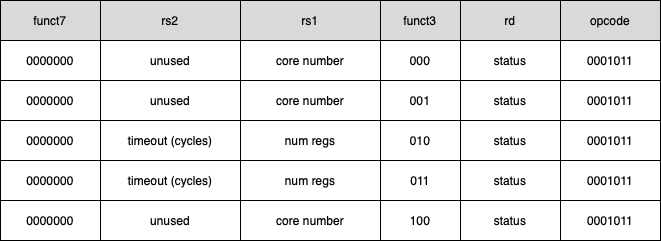
\includegraphics[width=1\linewidth]{figures/isa.png}
  \caption{RISC-V ISA Extensions}
  \label{fig:isa_extensions}
\end{figure}

\subsection{Software Design}

\subsubsection{Software Stack Overview}
To avoid nondeterministic latencies in the software stack, we need to minimize the use of the kernel \cite{Jia:ATC24:TraplessKprobes}. This means we cannot invoke system calls and kernel resources, as they utilize the trap, I/O, and scheduling that is out of the programmer's control.

We can do this by providing a set of user-space instructions that are exposed to the application programmer. These instructions can be used to configure FIFO buffers, send and receive data, and tear down FIFO buffers. 

We chose to use a polling mechanism to configure and tear down FIFO buffers. This is because polling, as opposed to interrupt-based, does not need the kernel and the programmer has full control over the frequency of polling. 

We modified the RISC-V toolchain and ISA \cite{Waterman:RISC-V:2019} to add the following instructions. The exact semantics of these instructions can be seen in Fig. \ref{fig:hw_ipc}
\begin{enumerate}
  \item \texttt{fconn}: Connect to a FIFO buffer
  \item \texttt{fcreate}: Create a FIFO buffer
  \item \texttt{fsend}: Write to a FIFO buffer
  \item \texttt{frecv}: Read from a FIFO buffer
  \item \texttt{fclose}: Close a FIFO buffer
\end{enumerate}

We provide a modified toolchain and compiler to be able to support these instructions natively.

\subsubsection{Configurability}
RVipc also allows a much more configurable data-flow path for the application programmer. A typical data-flow path may follow 

\begin{equation}
  \texttt{mem} \rightarrow \texttt{GPR} \rightarrow \texttt{FIFO} \rightarrow \texttt{GPR} \rightarrow \texttt{mem}
\end{equation}

But, for memory-independent, compute-bound, or sufficiently small workloads, the programmer can utilize
\begin{equation}
  \texttt{GPR} \rightarrow \texttt{FIFO} \rightarrow \texttt{GPR} \rightarrow \texttt{mem}
\end{equation}
where the bulk of the processing happens from GPR communication. For example, synchronization primitives like mutexes or status structs require only a few bytes of data, which can be sent across four GPRs.

We believe this provides an edge in latency and compute bound tasks, as a higher degree of configurability can lead to more robust and reliable software. 

\subsubsection{Handshake Protocol}
The singular point of nondeterminism in RVipc is the setup of the FIFOs. This is due to limited hardware resources and the need for an arbitrator. Since each core polls to acquire a buffer, the FIFO \texttt{fconn} and \texttt{fcreate} instructions have nondeterministic latencies.

The following handshake protocol is used to correctly configure the buffers. Let Hart 0 be the producer and Hart 1 be the consumer.

\begin{enumerate}
  \item Hart 0 issues \texttt{fcreate}, which sends a request to the pool to initialize a FIFO queue.
  \begin{enumerate}
      \item If the request completes, \texttt{status} will show 0.
      \item If there are no available FIFOs, \texttt{status} will show \( 1 \ll \texttt{ERR\_NO\_FIFO\_AVAIL} \).
      \item If a FIFO already exists with the issued core, \texttt{status} will show \( 1 \ll \texttt{ERR\_FIFO\_EXISTS} \).
  \end{enumerate}
  
  \item There is no dependence on Hart 1 when setting up the FIFO queue.
  
  \item The FIFO pool automatically closes the FIFO if inactive for \texttt{INACTIVE\_THRESH} cycles.
  
  \item Hart 1 issues \texttt{fconn}, which sends a request to the pool to connect to a FIFO queue.
  \begin{enumerate}
      \item If the request completes, \texttt{status} will show 0. The FIFO is now ready to use.
      \item If there is no FIFO set up for the core, \texttt{status} will show \( 1 \ll \texttt{ERR\_NO\_FIFO\_CREATED} \).
      \item If the core has already set up a prior connection with the same core, \texttt{status} will show \\
        \( 1 \ll \texttt{ERR\_ALREADY\_INITIALIZED} \).


  \end{enumerate}
  
  \item Hart 0 polls the pool with \texttt{fstatus}, which sends back \texttt{status}.
  \begin{enumerate}
      \item \texttt{status} will include information if the handshake was successful, FIFO is ready, etc.
  \end{enumerate}
  
  \item Hart 1 polls the pool with \texttt{fstatus}, which sends back \texttt{status}.
  \begin{enumerate}
      \item \texttt{status} will include information if the handshake was successful, FIFO is ready, etc.
  \end{enumerate}
  
  \item Hart 0 is now able to send with \texttt{fsend}. Hart 1 is now able to receive with \texttt{frecv}.
\end{enumerate}


Note that Hart 0 and Hart 1 need to poll to set up the FIFO with \texttt{fstatus}. In a many-core system this can cause backpressure on the pool to service these instructions. However, the aim of polling is to allow \texttt{fstatus} to resolve by the end of the WriteBack stage, so as to not cause any pipeline stalls or increase critical path. This mechanism also avoids any kernel traps which further improves latency.


\subsection{Implementation}
We utilized Gem5 to implement the hardware FIFO pool. There is a global class \texttt{HwIpc}, which contains the necessary data mappings for the FIFO pool and appropriate locking mechanisms to ensure proper simulation. 

We configured the simulated machine to have a dual core system. This is sufficient as we are testing latencies in sending and receiving data, not FIFO setup contention. 

Each core has an instruction and data cache. Each cache is connected to the memory controller. The exact Gem5 configuration we utilized is attached in Fig. \ref{fig:gem5}.

\begin{figure}[h]
  \centering
  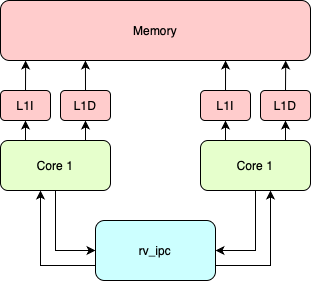
\includegraphics[width=0.6\linewidth]{figures/hardware.png}
  \caption{Architectural overview of Gem5 simulation, including the FIFO pool, CPU cores, caches, and memory controller.}
  \label{fig:hw_ipc}
\end{figure}

\begin{figure}[h]
  \centering
  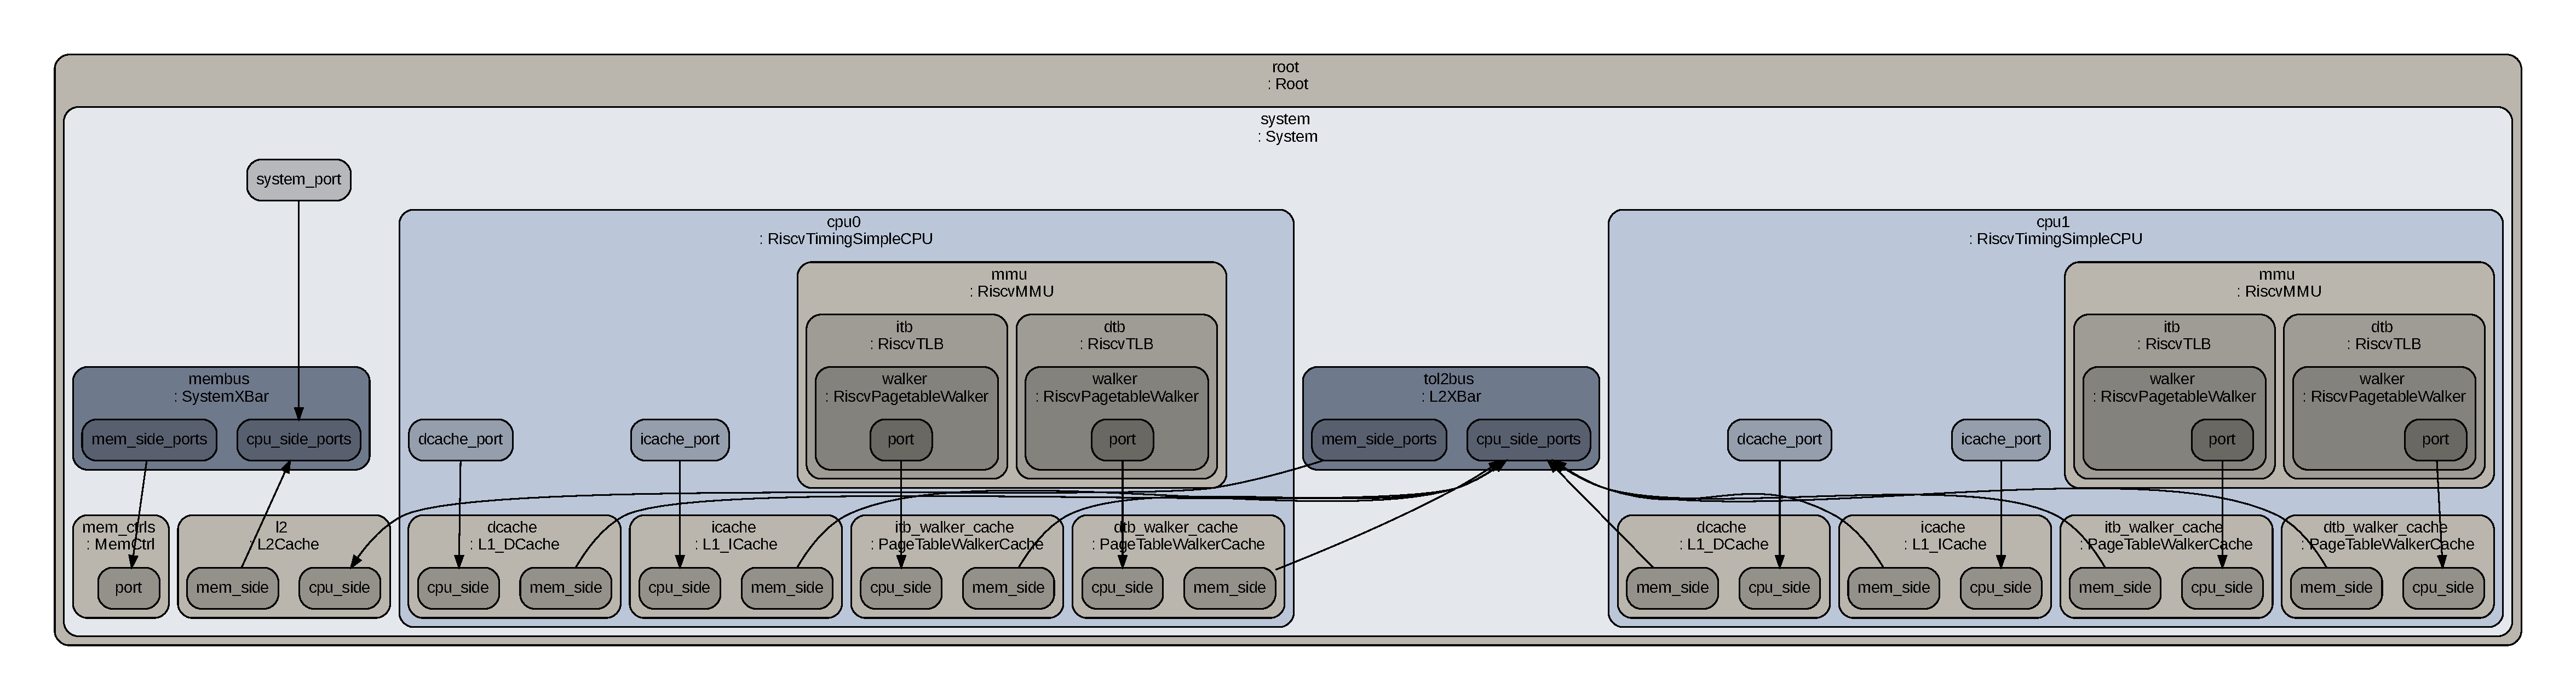
\includegraphics[width=1.0\linewidth]{figures/gem5.pdf}
  \caption{Gem5 configuration setup.}
  \label{fig:gem5}
\end{figure}

The following is an example of the command used to run the simulation:
\begin{verbatim}
  build/RISCV/gem5.fast --outdir=m5out/ \
  configs/deprecated/example/se.py \
  --cpu-type=RiscvTimingSimpleCPU --num-cpus=2 \
  --redirects /lib=/home/fluxbyt/riscv-compiled/lib \
  --cpu-clock=4GHz \
  --cacheline_size=64 \
  --caches \
  --l1i_size=8kB \
  --l1d_size=8kB \
  --l2cache \
  --l2_size=4MB \
  --l2_assoc=16 \
  --cmd="ipc_bin/test_send;ipc_bin/test_recv"
\end{verbatim}

\subsection{Parameter Sweep}

After designing an appropriate hardware and software architecture for the FIFO pool, we ran an extensive design space exploration to realize under which conditions our system performs best. 

\subsubsection{First Message Latency}
The first message latency is defined as the time from the first packet of data sent to the first packet of data received.

\begin{figure}[h]
  \centering
  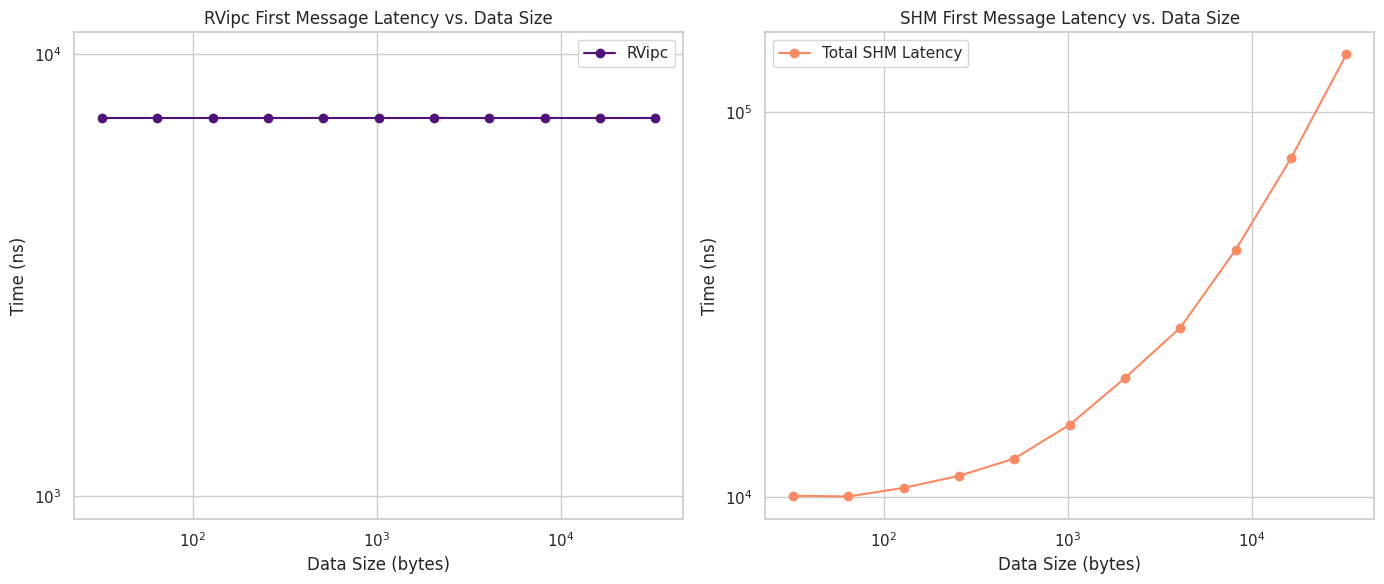
\includegraphics[width=1\linewidth]{figures/first-message-lat.png}
  \caption{First message latency of RVipc and SHM.}
  \label{fig:first_byte_latency}
\end{figure}

The first message latency of the shared memory mechanism scales as the size of the data increases. However, RVipc maintains constant latency. This is key in ensuring deterministic latency behavior for the set of applications we are targeting.

\subsubsection{Overall Latency}
RVipc has a constant first message latency, and linear latency for data size as indicated in Fig. \ref{fig:first_byte_latency}. Let $\texttt{NUM\_CYCLES}$ denote the number of cycles for a single packet of data to be sent. By definition, this is constant as we have a dedicated FIFO link between the communicating cores. Let \texttt{NUM\_SETUP} denote the number of cycles required to create and set up the FIFO. Additionally, let \texttt{N} denote the number of packets we are sending.



The overall latency is then defined as:
\begin{equation}
  \texttt{latency} = \texttt{NUM\_SETUP} + \texttt{NUM\_CYCLES} \cdot \texttt{N}
\end{equation}

This further ensures deterministic latencies. 

Contrastingly, we note that SHM has unpredictable latencies, even when broken into the read and write latency separately. Additionally, there is a large benefit to using RVipc for either low-latency first messages, or relatively small amounts of data. 

\begin{figure}[h]
  \centering
  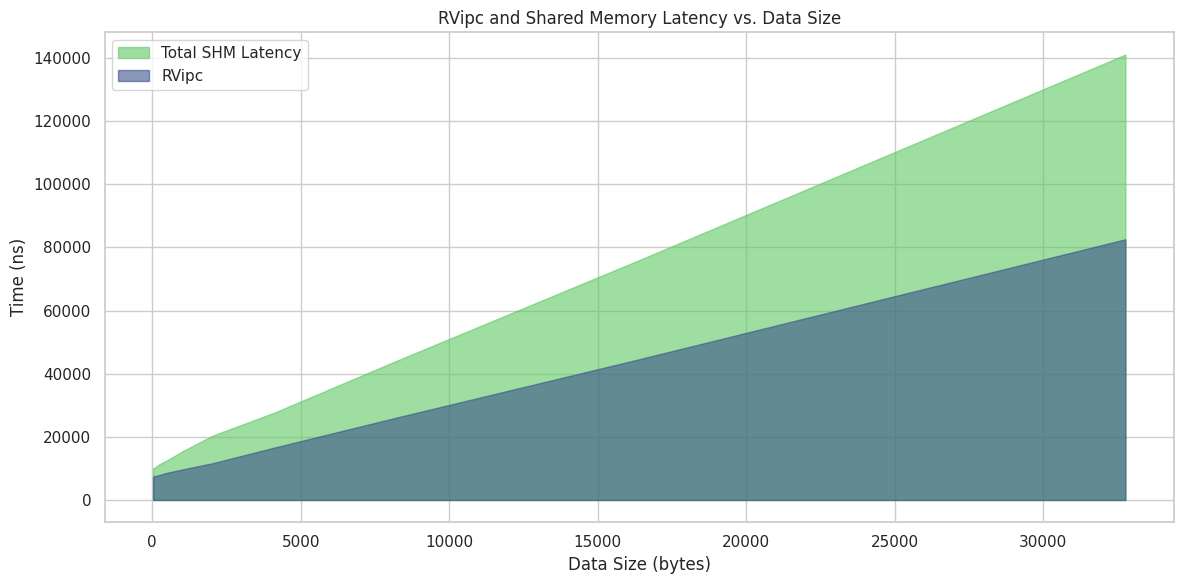
\includegraphics[width=1\linewidth]{figures/lat-v-dat.png}
  \caption{Overall latency comparison of RVipc and SHM.}
  \label{fig:overall_latency}
\end{figure}

\subsubsection{Bandwidth}
While the latency of the system is the primary focus of this work, the bandwidth, or throughput, of the FIFO pool is just as crucial. We note that, as indicated in Fig. \ref{fig:bandwidth}, that RVipc successfully surpasses the shared memory bandwidths for sufficiently large data sizes.

Though this does not take into account contention on the FIFO pool for sending data, it is a reasonable approximation that RVipc will not harm bandwidth, if not improve it.

\begin{figure}[h]
  \centering
  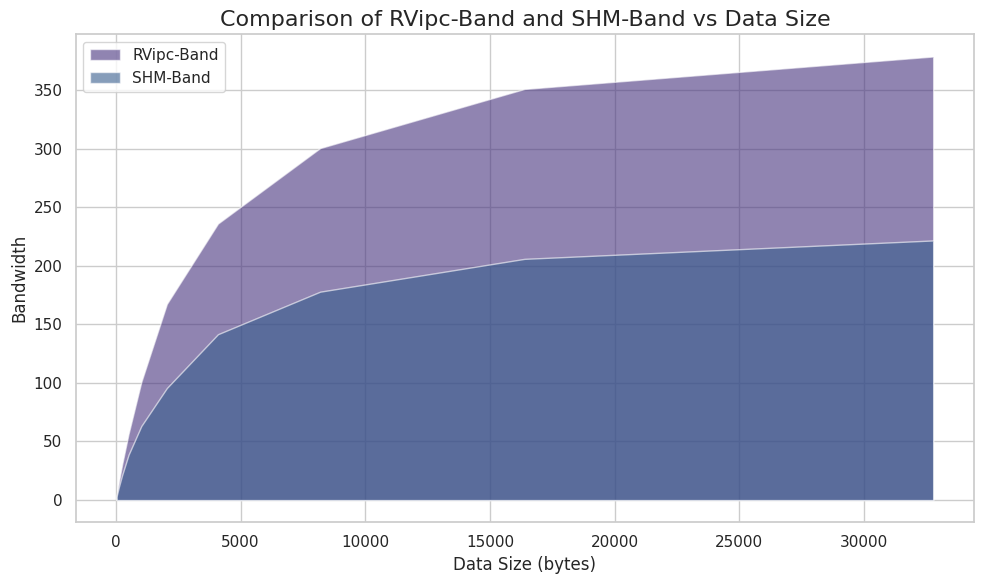
\includegraphics[width=1\linewidth]{figures/band-v-dat.png}
  \caption{Bandwidth comparison of RVipc and SHM.}
  \label{fig:bandwidth}
\end{figure}

\subsubsection{Cache Line}

The last parameter we sweeped is the cache line size. The reason for exploring this parameter is because being able to send data in larger chunks has direct implications on cache pollution and message latencies. As indicated in Fig. \ref{fig:cache_line}, RVipc yields lower latencies and higher throughptus for larger cache lines. This provides valuable insight into what kinds of cache hierarchies are appropriate for RVipc.

\begin{figure}[h]
  \centering
  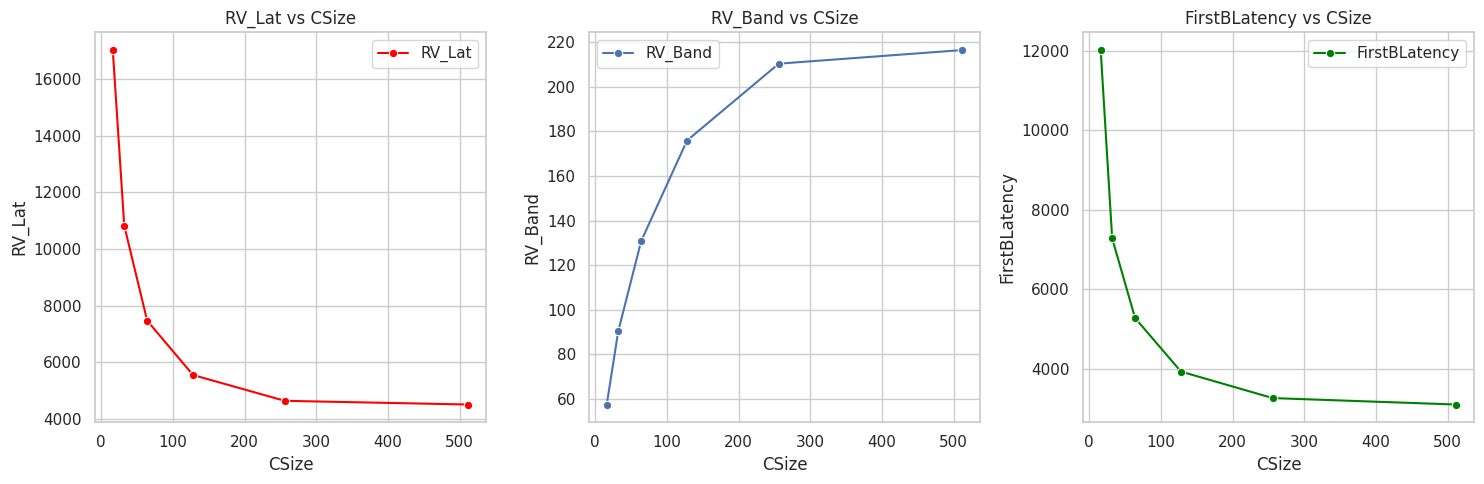
\includegraphics[width=1\linewidth]{figures/band-v-linesz.png}
  \caption{Bandwidth vs. Cache Line Size Comparison of RVipc and SHM.}
  \label{fig:cache_line}
\end{figure}

\subsection{Cache Pollution and Latency Analysis}
\subsubsection{Cache Pollution}
We define cache pollution as the amount of cache evictions that are caused by a shared memory read-write operation. Concretely, let $M_{L_2}$ denote the amount of lines evicted from the L2 cache when reading $M$. Let $M_{L_1D}$ denote the lines evicted when bringing data into the L1 data cache. Let $M'_{L_1D}$ and $M'_{L_2}$ denote the amount of lines that we want to share between the cores from L1 data and L2, respectively.

We conduct our theoretical analysis on a non-includsive eviction policy, as modern systems like Intel and Apple silicon utilize this policy.

\begin{equation}
  \texttt{pollution}_{SHM} = M_{L_2} + M_{L_1D} + M'_{L_1D_0} + M'_{L_2} + M'_{L_1D_1}
\end{equation}

However, RVipc does not need to put $M'$ into cache and can directly utilize the FIFOs. Therefore, 

\begin{equation}
  \texttt{pollution}_{RVipc} = M_{L_2} + M_{L_1D} + M'_{L_1D_1}
\end{equation}

Note that RVipc always yields less cache pollution that SHM, specifically by $M'_{L_1D_0} + M'_{L_2}$. This is important to minimize latency variation in the system. The larger the amount of data being transferred over shared memory is, the more pollution the mechanism causes and the better RVipc performs.

\subsubsection{Latency Analysis}
Let $\theta_{L_2}$ be the time required to bring $M$ lines into the L2 cache. Let $\theta_{L_1}$ be the time required to bring $M$ lines into the L1 data cache from the L2 cache. Let $\alpha_{L_1}$ be the time required to put $M$ lines from L1 data into L2. Let $\beta$ denote the time required to send a single message via the FIFO buffers.

\begin{equation}
  \texttt{latency}_{SHM} = \theta_{L_2} + \theta_{L_1} + \alpha_{L_1} + \theta_{L_1}
\end{equation}

\begin{equation}
  \texttt{latency}_{RVipc} = \theta_{L_2} + \theta_{L_1} + M \cdot \beta
\end{equation}

Notice that as long as $M \cdot \beta < \alpha_{L_1} + \theta_{L_1}$, RVipc will yield lower latencies than SHM. The performance implications of SHM over RVipc is hardware depedendent.

\section{Security Considerations}
\subsection{Current Security Protections}
While RVipc is designed for trusted environments, the system does incorporate security principles to ensure a certain level of robustness.

Side-channel attacks take advantage of system metrics that are data dependent to decode information about the inputs. Because RVipc operates on GPRs, the FIFO send and recieves are constant time operations. Constant time operations make it resilient to timing side-channel attacks as an attacker cannot learn information about the input from send/recieve timing. Furthermore, to correctly setup a FIFO, both the sending and recieving Harts need to agree on a secret key. This prevents a malicious thread on a Hart from accessing a FIFO being used by a different thread on the same Hart.

\subsection{Future Security Extensions}
Currently, the FIFO keys are configurable keys. A future extension would be to introduce a kernel control status register (CSR) to configure how the keys are generated and used.